\documentclass[tikz, border=5pt]{standalone}

\newcommand{\threshdraw}[3]{%
  \draw[->] (#1) --
    node[pos=0.45] {\tikz \fill (0,0) -- (0.4,0.6) -- (-0.4,0.6) -- cycle;}
    node[pos=0.45, xshift=20pt] {\LARGE $\tau_{#3}$}
  (#2);
}

\usepackage{tikz}
\usetikzlibrary{
  arrows.meta,
  calc,
  positioning,
  shapes.geometric,
  shadows.blur,
  bending,
  decorations.markings
}

\begin{document}
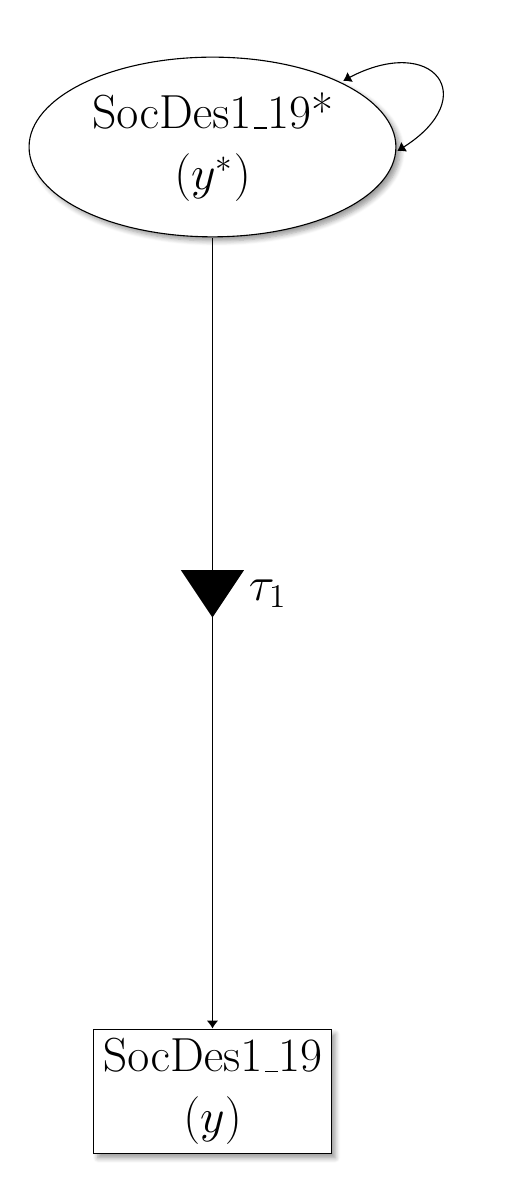
\begin{tikzpicture}

\tikzset{
  threshold/.style n args={1}{
  postaction={
    decorate,
    decoration={
      markings,
      mark=at position 0.5 with {
        \fill (0,0) -- (0.2,0.3) -- (-0.2,0.3) -- cycle;
        \node[xshift=15pt] {\LARGE $#1$};
      }
    }
  }
},
  socdesyear/.style={
    draw,
    ellipse,
    fill=white,
    % minimum width=2.6cm,
    % minimum height=0.9cm,
    align=center,
    font = \LARGE,
    blur shadow={shadow xshift=1.5pt, shadow yshift=-1.5pt, shadow blur steps=6}
},
  observ/.style={
    draw,
    rectangle,
    fill=white,
    % minimum width=2.8cm,
    % minimum height=1.1cm,
    align=center,
    font=\LARGE,
    blur shadow={shadow xshift=1.5pt, shadow yshift=-1.5pt, shadow blur steps=6}
  },
  >={Latex[length=1mm, width=1.5mm]},
  line width=1pt
}

% NODES ----------------------------------------------------------

% Nodes SocDes Star (use the same style of `socdesyear`) + Dots
\node[socdesyear] (y1star)   at (0   , 12)   {SocDes1\_19* \\ $(y^{*})$};

% Nodes categorical observed variables
\node[observ] (y1)   at (0,    0) {SocDes1\_19 \\ $(y)$};

% DRAWS ---------------------------------------------------------

% Draws latent categorical + triangle
\threshdraw{y1star}{y1}{1}

%% Variance
\draw[<->]
($(y1star.north east)+(0.00,0.02)$)
to[out=30, in=30, looseness=3]
($(y1star.east)+(0,-0.05)$);

\end{tikzpicture}
\end{document}